% chapter03.tex

 %%%%%%%%%%%%%%%%%%%%%%%%%%%%%%%%%%%%%%%%%%%%%%%%%%%%%%%%%%%%%%%%%%%%%%%%%%%%%
 %                                                                           %
 %    PyMS documentation                                                     %
 %    Copyright (C) 2005-2010 Vladimir Likic                                 %
 %                                                                           %
 %    The files in this directory provided under the Creative Commons        %
 %    Attribution-NonCommercial-NoDerivs 2.1 Australia license               %
 %    http://creativecommons.org/licenses/by-nc-nd/2.1/au/                   %
 %    See the file license.txt                                               %
 %                                                                           %
 %%%%%%%%%%%%%%%%%%%%%%%%%%%%%%%%%%%%%%%%%%%%%%%%%%%%%%%%%%%%%%%%%%%%%%%%%%%%%

\chapter{GC-MS data derived objects}

In the raw GC-MS data, consecutive scans do not necessarily contain the same
mass per charge (mass) values. For data processing, it is often necessary to
convert the data to a matrix with a set number of masses and scans. In PyMS,
the resulting object is called intensity matrix. In this chapter the methods
for converting the raw GC-MS data to an intensity matrix object are illustrated.

\section{\label{sec:intensity-matrix}IntensityMatrix Object}
The general scheme for converting raw mass values is to bin intensity values
based on the interval the corresponding mass belongs to. The general procedure
is as follows:
\begin{itemize}
    \item Set the interval between bins, lower and upper bin boundaries
    \item Calculate the number of bins to cover the range of all masses.
    \item Centre the first bin at the minimum mass found for all the raw data.
    \item Sum intensities whose masses are in a given bin.
\end{itemize}

A mass, $m$, is considered to belong to a bin when $c - l \le m < c + u$,
where $c$ is the centre of the bin, $l$ is the lower boundary and $u$ is
the upper boundary of the bin. The default bin interval is one with a lower
and upper boundary of $\pm0.5$.

A function to bin masses to the nearest integer is also available. The default
bin interval is one with a lower boundary of -0.3 and upper boundary of +0.7 (as
per the NIST library).

% Figure~\ref{fig:binning} illustrates the process of assigning bins to the mass
% axis and summing all intensities in a given bin. The result is a new mass axis
% with mass values corresponding to the centre of each bin.

% \begin{figure}[htp]
% \begin{center}
% %\includegraphics{graphics/binning/binning.eps}
% \caption{Mass intensity values are added to bins based on a pre-set bin size
%and
% the minimum mass of all the scan data. All intensities in a given bin width
% (top) are added and given a mass of the centre of the bin (bottom). For
%integer
% binning, each bin has a width of one and is centred at integer values.}
% \label{fig:binning}
% \end{center}
% \end{figure}

\subsection{Discussion of Binning Boundaries}

For any chemical element $X$, let $w(x)$ be the atomic weight of $X$, and

\begin{equation}
\delta(X) = \frac{w(X) - \{w(X)\}}{w(X)}, 
\end{equation}

where $\{a\}$ is the integer value of $a$ (rounded to the nearest integer).

For example, for hydrogen $\delta(^1\rm{H}) = \frac{1.007825032 - 1}{1.007825032} = 
0.0076$. Similarly $\delta(^{12}\rm{C}) = 0$, $ \delta(^{14}\rm{N}) = 0.00022$,
$\delta(^{16}\rm{O}) = -0.00032$, etc.

Let also $\Delta(X) = w(X) - \{w(x)\}$. Then $-0.023 <\Delta(^{31}\rm{P}),
\Delta(^{28}\rm{Si}) < 0$.

Let a compound undergo GC-MS and let Y be one of it's fragments. If Y consists 
of $k_{1}$atoms of type $X_{1}$, 
$k_{2}$ atoms of type $X_{2}$,....., 
$k_{r}$ atoms of type $X_{r}$, then
$\Delta(Y) = k_{1}*\Delta(X_{1}) + k_{2}*\Delta(X_{2}) + ....+ k_{r}*
\Delta(X_{r})$.

The fragment will usually not contain more than 2 or 3 P or Si atoms and if it's 
molecular weight is less than 550 it may not contain more than 35 O atoms, so 
$\Delta(Y) \geq -0.023*5 - 0.00051*35 = -0.133$.

On the other hand, of Y contains $k$ H atoms and $m$ N atoms, then $\Delta(Y)
\leq k*0.00783 + m*0.00051$. Since for each two hydrogen atoms at least one
carbon (or heavier) atom is needed, giving the limit of no more than 80 hydrogen
atoms. Therefore in this case (i.e. H and C atoms only)$\Delta(Y) \leq 80*0.00783
= 0.63$. If carbon is replaced by any heavier atom, at least 2 hydrogen atoms
will be eliminated and $\Delta(Y)$ will become even smaller.

If the molecular weight of $Y$ does not exceed 550 (typically the largest mass
scanned for in a GC-MS setup) then $\mathbf{-0.133 \leq \Delta(Y) \leq 0.63}$.
This means that if we set our binning boundaries to $(-0.3, 0.7)$ or $(-0.2, 0.8)$
the opportunity for having a fragment whose molecular weight is very close to
the boundary is minimised.

Since the resolution of MS is at least 0.1 dalton, we may assume that it's error
does not exceed 0.05, and MS accuracy will not cause additional problems.

\subsection{Build intensity matrix}

\noindent
[ {\em This example is in pyms-test/30a} ]

An intensity matrix on the raw GC-MS data can be built using the following
function. First the raw data is imported as before.

\begin{verbatim}
>>> from pyms.GCMS.IO.JCAMP.Function import JCAMP_reader
>>> jcamp_file = "/x/PyMS/data/gc01_0812_066.jdx"
>>> data = JCAMP_reader(jcamp_file)
 -> Reading JCAMP file '/x/PyMS/pyms-data/gc01_0812_066.jdx'
>>>
\end{verbatim}

\noindent
Then the data can be converted to an intensity matrix using the functions
{\tt build\_intensity\_matrix()} and {\tt build\_intensity\_matrix\_i()},
available in ``pyms.GCMS.Function''.

The default operation of {\tt build\_intensity\_matrix()} is to use a bin
interval of one and treat the masses as floating point numbers. The default
intensity matrix can be built as follows:

\begin{verbatim}
>>> from pyms.GCMS.Function import build_intensity_matrix
>>> im = build_intensity_matrix(data)
\end{verbatim}

The size as the number of scans and the number of bins is returned by:
\begin{verbatim}
>>> im.get_size()
(9865, 551)
\end{verbatim}

There are 9865 scans and 551 bins in this example.

The raw masses have been binned into new mass units based on the minimum mass
in the raw data and the bin size. A list of the new masses can be obtained
as follows:

\begin{verbatim}
>>> masses = im.get_mass_list()
>>> print masses[:10]
[50.0, 51.0, 52.0, 53.0, 54.0, 55.0, 56.0, 57.0, 58.0, 59.0]
\end{verbatim}

The last command prints the first ten masses. The methods {\tt im.get\_min\_mass()}
and {\tt get\_max\_mass()} return the minimum and maximum mass:

\begin{verbatim}
>>> print im.get_min_mass()
50.0
>>> print im.get_max_mass()
600.0
\end{verbatim}

It is also possible to search for a particular mass, by finding the index of
the binned mass closest to the desired mass. For example, the index of the
closest binned mass to a mass of 73.3 m/z can be found by using the
methods {\tt get\_index\_of\_mass()}:

\begin{verbatim}
>>> index = im.get_index_of_mass(73.3)
>>> print index
23
\end{verbatim}

The value of the closest mass can be returned by the method
{\tt get\_mass\_at\_index()}:

\begin{verbatim}
>>> print im.get_mass_at_index(index)
73.0
\end{verbatim}

A mass of 73.0 is returned in this example.

\subsection{Build intensity matrix parameters}

\noindent
[ {\em This example is in pyms-test/30b} ]

The bin interval can be set to values other than one, and binning boundaries
can also be adjusted. In the example below, to fit the 0.5 bin interval, the
upper and lower boundaries are set to $\pm$0.25.

\begin{verbatim}
im = build_intensity_matrix(data, 0.5, 0.25, 0.25)
\end{verbatim}

The size of the intensity matrix will reflect the change in the number of bins:

\begin{verbatim}
>>> im.get_size()
\end{verbatim}

In this example there are 9865 scans (as before), but 1101 bins.

The index and binned mass of the mass closest to 73.3 should also reflect the
different binning.

\begin{verbatim}
>>> index = im.get_index_of_mass(73.3)
>>> print im.get_mass_at_index(index)
\end{verbatim}

A mass of 73.5 is returned in this example.

\subsection{Build integer mass intensity matrix}

\noindent
[ {\em This example is in pyms-test/30c} ]

It is also possible to build an intensity matrix with integer masses and a bin
interval of one. The default range for the binning is -0.3 and +0.7 mass
units. The function is imported from ``pyms.GCMS.Function'':

\begin{verbatim}
>>> from pyms.GCMS.Function import build_intensity_matrix_i
>>> im = build_intensity_matrix_i(data)
\end{verbatim}

The masses are now integers.

\begin{verbatim}
>>> index = im.get_index_of_mass(73.3)
>>> print im.get_mass_at_index(index)
\end{verbatim}

A mass of 73 is returned in this example.

The lower and upper bounds can be adjusted by {\tt
build\_intensity\_matrix\_i(data, lower, upper)}.

\section{MassSpectrum object}

\noindent
[ {\em This example is in pyms-test/31} ]

\noindent
A MassSpectrum object contains two attributes, {\tt mass\_list} and
{\tt mass\_spec}, a list of mass values and corresponding intensities,
respectively. MassSpectrum is returned by the IntensityMatrix method
{\tt get\_ms\_at\_index(index)}.

For example, the properties of the first MassSpectrum object of an
IntensityMatrix, {\em im}, can be investigated by;

\begin{verbatim}
>>> ms = im.get_ms_at_index(0)
>>> print len(ms)
>>> print len(ms.mass_list)
>>> print len(ms.mass_spec)
\end{verbatim}

\noindent
The length of all attributes should be the same.

\section{IonChromatogram object}
\label{sec:ion-chromatogram-object}
\noindent
[ {\em This example is in pyms-test/31} ]

\noindent
An IonChromatogram object is a one dimensional vector containing
mass intensities as a function of retention time. This can can be either
m/z channel intensities (for example, the ion chromatogram at m/z = 73),
or cumulative intensities over all measured m/z (TIC).

An IonChromatogram for the TIC and a given mass or index can be obtained
as follows:

\begin{verbatim}
>>> tic = data.get_tic()
>>> ic = im.get_ic_at_index(0)
>>> ic = im.get_ic_at_mass(73)
\end{verbatim}

\noindent
This will return, respectively: the TIC; the ion chromatogram of the first
mass; and the ion chromatogram of the mass closest to 73.

An ion chromatogram object has a method {\tt is\_tic()} which returns "True"
if the ion chromatogram is a TIC, "False" otherwise:

\begin{verbatim}
>>> print "'tic' is a TIC:", tic.is_tic()
'tic' is a TIC: True
>>> print "'ic' is a TIC:",ic.is_tic()
'ic' is a TIC: False
\end{verbatim}

\subsection{Writing IonChromatogram object to a file}

\noindent
[ {\em This example is in pyms-test/31} ]

The method {\tt write()} of IonChromatogram object allows one to save
the ion chromatogram object to a file:

\begin{verbatim}
>>> tic.write("output/tic.dat", minutes=True)
>>> ic.write("output/ic.dat", minutes=True)
\end{verbatim}

\noindent
The flag minutes=True indicates that retention time will be saved in minutes.
The ion chromatogram object saved with with the {\tt write{}} method is a
plain ASCII file which contains a pair of (retention time, intensity) per
line.

\begin{verbatim}
$ head tic.dat
  5.0930 2.222021e+07
  5.0993 2.212489e+07
  5.1056 2.208650e+07
  5.1118 2.208815e+07
  5.1181 2.200635e+07
  5.1243 2.200326e+07
  5.1306 2.202363e+07
  5.1368 2.198357e+07
  5.1431 2.197408e+07
  5.1493 2.193351e+07
\end{verbatim}

% \noindent
% Figure \ref{fig:tic-plot} shows the plot of the file 'tic.dat' produced with
% the program Gnuplot.
%
% \begin{figure}[htp]
% \begin{center}
% %x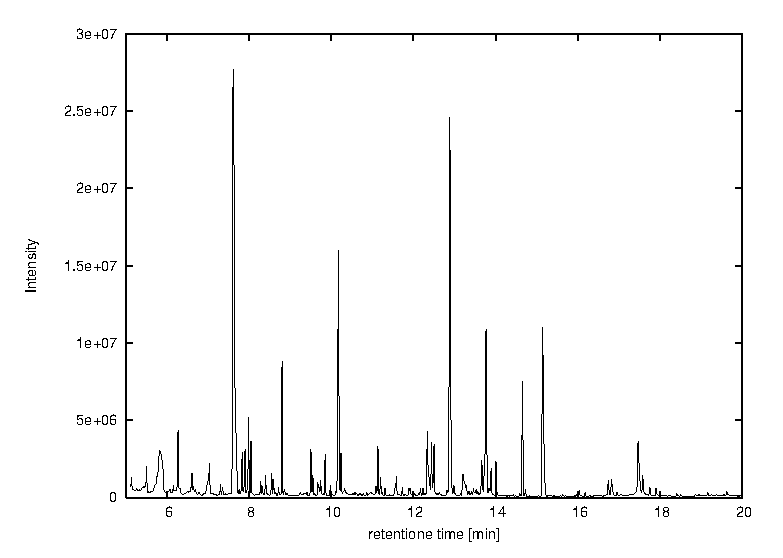
\includegraphics{graphics/pyms-test/tic.eps}
% \caption{The Gnuplot plot of the file 'tic.dat'}
% \label{fig:tic-plot}
% \end{center}
% \end{figure}

\section{Saving data}

\noindent
[ {\em This example is in pyms-test/32} ]

\noindent
A matrix of intensity values can be saved to a file with the function
{\tt save\_data()} from {\tt pyms.Utils.IO}. A matrix of intensity values can
be returned from an IntensityMatrix with the method {\tt get\_matrix\_list()}.
For example,

\begin{verbatim}
>>> from pyms.Utils.IO import save_data
>>> mat = im.get_matrix_list()
>>> save_data("output/im.dat", mat)
\end{verbatim}

It is also possible to save the list of masses (from {\tt im.get\_mass\_list()})
and the list of retention times (from {\tt im.get\_time\_list()}) using the
{\tt save\_data()} function. For convenience, the intensity values, mass list
 and time list, can be saved with the method {\tt export\_ascii()}. For example,

\begin{verbatim}
>>> im.export_ascii("output/data")
\end{verbatim}

\noindent
will create ``data.im.dat'', ``data.mz.dat'', and ``data.rt.dat'' where these
are the intensity matrix, retention time vector, and m/z vector. By default
the data is saved as space separated data with a ``.dat'' extension. It is
also possible to save the data as comma separated data with a ``.csv''
extension by the command ``{\tt im.export\_ascii("output/data", "csv")}''.

Additionally, the entire IntensityMatrix can be exported to LECO CSV format.
This facility is useful for import into other analytical software packages.
The format has a header line specifying the column heading information as:
``scan, retention time, mass1, mass2, $\dots$'', and then each row as the
intensity data.

\begin{verbatim}
>>> im.export_leco_csv("output/data_leco.csv")
\end{verbatim}

\section{Importing ASCII data}

\noindent
[ {\em This example is in pyms-test/32} ]

The LECO CSV data format can be used to import ASCII data directly into an
IntensityMatrix object.  The data must follow the format outlined above.
For example, the file saved above can be read and compared to the original:

\begin{verbatim}
>>> from pyms.GCMS.Class import IntensityMatrix
>>>
>>> iim = IntensityMatrix([0],[0],[[0]])
>>>
>>> iim.import_leco_csv("output/data_leco.csv")
>>>
>>> print im.get_size()
>>> print iim.get_size()
\end{verbatim}

The line ``IntensityMatrix([0],[0],[[0]])'' is required to create an empty
IntensityMatrix object.

